
\documentclass[letterpaper, reqno,11pt]{article}
\usepackage[margin=1.0in]{geometry}
\usepackage{color,latexsym,amsmath,amssymb}
\usepackage{fancyhdr}
\usepackage{amsthm}
\usepackage[linesnumbered,lined,boxed,commentsnumbered,noend,noline]{algorithm2e}
\usepackage{dsfont}
\usepackage{graphicx}
\usepackage{hyperref}
\usepackage{bbm}
\usepackage[inline]{enumitem}
\usepackage[numbers]{natbib}
\usepackage{framed}
\usepackage{titling}
\usepackage{subcaption}
\usepackage[dvipsnames]{xcolor}
\usepackage{tikz}

\tikzset{invclip/.style={clip,insert path={{[reset cm]
  (-16383.99999pt,-16383.99999pt) rectangle (16383.99999pt,16383.99999pt)}}}}

\allowdisplaybreaks

\newcommand{\RR}{\mathbb{R}}
\newcommand{\CC}{\mathbb{C}}
\newcommand{\ZZ}{\mathbb{Z}}
\newcommand{\QQ}{\mathbb{Q}}
\newcommand{\NN}{\mathbb{N}}
\newcommand{\FF}{\mathbb{F}}
\newcommand{\PP}{\mathbb{P}}
\newcommand{\EE}{\mathbb{E}}
\newcommand{\LL}{\mathbb{L}}
\newcommand{\TT}{\mathbb{T}}
\newcommand{\GI}{\textrm{GI}}
\newcommand{\coGI}{\overline{\textrm{GI}}}
\DeclareMathOperator{\conv}{conv}
\DeclareMathOperator{\charcone}{char.cone}
\DeclareMathOperator{\STAB}{STAB}
\DeclareMathOperator{\Down}{Down}
\DeclareMathOperator{\lca}{lca}
\DeclareMathOperator{\ex}{ex}
\DeclareMathOperator{\Span}{span}
\DeclareMathOperator{\T}{T}
\DeclareMathOperator{\F}{F}
\DeclareMathOperator{\shP}{\# P}
\DeclareMathOperator{\shSAT}{\# SAT}
\DeclareMathOperator{\shDNF}{\# DNF}
\DeclareMathOperator{\DNF}{DNF}
\DeclareMathOperator{\Poly}{P}
\DeclareMathOperator{\CNF}{CNF}
\DeclareMathOperator{\SAT}{SAT}
\DeclareMathOperator{\BPP}{BPP}
\DeclareMathOperator{\poly}{poly}
\DeclareMathOperator{\RP}{RP}
\DeclareMathOperator{\EXP}{EXP}
\DeclareMathOperator{\DTIME}{DTIME}
\DeclareMathOperator{\NP}{NP}
\DeclareMathOperator{\MCprime}{MC'}
\DeclareMathOperator{\Var}{Var}
\DeclareMathOperator{\IP}{IP}
\DeclareMathOperator{\PSPACE}{PSPACE}
\DeclareMathOperator{\lollipop}{lollipop}
\DeclareMathOperator{\ustconn}{\textsc{UST-Conn}}
\DeclareMathOperator{\RL}{RL}
\newcommand\mycommfont[1]{\ttfamily\textcolor{blue}{#1}}
\SetCommentSty{mycommfont}
\begin{document}
\pagenumbering{arabic}
\title{Lectures on Random Walks}
\author{Yuchong Pan}
\date{\today}
\newtheorem{theorem}{Theorem}
\newtheorem{lemma}[theorem]{Lemma}
\newtheorem{proposition}[theorem]{Proposition}
\newtheorem{corollary}[theorem]{Corollary}
\newtheorem{fact}[theorem]{Fact}
\newtheorem{problem}[theorem]{Problem}
\newtheorem{claim}{Claim}
\newtheorem{exercise}{Exercise}
\theoremstyle{definition}
\newtheorem{definition}[theorem]{Definition}
%\maketitle
%

\begin{framed}
\noindent{\bf 6.842 Randomness and Computation} \hfill \thedate
\begin{center}
\Large{\thetitle}
\end{center}
\noindent{\em Lecturer: Ronitt Rubinfield} \hfill {\em Scribe: \theauthor}
\end{framed}

\section{Markov Chains and Random Walks}

\begin{definition}
  Let $\Omega$ be a set of states (throughout this note, $\Omega$ is finite). A sequence of random walks $X_0, X_1, \ldots \in \Omega$ is a \emph{Markov chain} if it satisfies the \emph{Markovian property}, i.e., for each $t \in \NN$ and for all $x_1, \ldots, x_t, y \in \Omega$,
  $$ \PP\left[X_{t + 1} \;\middle|\; X_1 = x_1, \ldots, X_t = x_t\right] = \PP\left[X_{t + 1} = y \;\middle|\; X_t = x_t\right]. $$
  WLOG, we assume that transitions are independent of time. For $x, y \in \Omega$, let
  $$ P(x, y) = \PP\left[X_{t + 1} = y \;\middle|\; X_t = x\right]. $$
  Interpreted as a matrix, $P$ is called the \emph{transition matrix} of the Markov chain. We can also interpret the transition matrix $P$ as a weighted directed graph with vertex set $\Omega$ such that the weight on $(i, j) \in \Omega^2$ equals $P(i, j)$.
\end{definition}

A random walk on a directed graph is a special case of Markov chains.

\begin{definition}
  A \emph{random walk} on a directed graph $G = (V, E)$ is a sequence $S_1, S_2, \ldots \in V$ such that $S_{t + 1}$ is picked uniformly in $N^+(S_t)$, i.e., the transition matrix $P$ is defined so that for $x, y \in V$,
  $$ P(x, y) = \left\{
    \begin{array}{ll}
      \frac{1}{d^+(x)}, & \text{if $(x, y) \in E$}, \\
      0, & \text{otherwise}.
    \end{array}
  \right. $$
\end{definition}

\begin{definition}
  Let $P$ be an $n \times n$ matrix. Then $P$ is said to be \emph{stochastic} if for all $i \in [n]$,
  $$ \sum_{j = 1}^n P(i, j) = 1. $$
  Moreover, $P$ is said to be \emph{doubly stochastic} if $P$ is stochastic and for all $j \in [n]$,
  $$ \sum_{i = 1}^n P(i, j) = 1. $$
\end{definition}

For each $t \in \NN$, let $P_t(x, y)$ ve the transition probability from $x$ to $y$ for $t$ steps. Then for all $x, y \in \Omega$ and $t \in \NN$,
$$ P^t(x, y) = \left\{
  \begin{array}{ll}
    P(x, y), & \text{if $t = 1$}, \\
    \sum_{z \in \Omega} P(x, z) P^{t - 1}(z, y) & \text{if $t > 1$}.
  \end{array}
\right. $$
Interpreted as matrix multiplication, for each $t \in \NN$ with $t > 1$,
$$ P^t = P \cdot P^{t - 1}. $$
Let $\pi^{(0)} = (\pi_1^{(0)}, \ldots, \pi_n^{(0)})$ be the initial distribution, where $\pi_i^{(0)}$ is the probability of starting at vertex $i$ for each $i \in [n]$.\footnote{WLOG, we assume $\Omega = [n]$.} Let $\pi^{(t)}$ be the distribution after $t$ steps for each $t \in \NN$. For each $t \in \NN$,
$$ \pi^{(t)} = \pi^{(0)} P^t. $$

\begin{definition}
  A distribution $\pi^*$ is called a \emph{stationary distribution} of a Markov chain with state set $\Omega$ and transition matrix $P$ if for all $x \in \Omega$,
  $$ \pi^*(x) = \sum_{y \in \Omega} \pi^*(y) P(y, x). $$
\end{definition}

\begin{definition}
  A Markov chain with state set $\Omega$ and transition matrix $P$ is said to be \emph{irreducible} if for all $x, y \in \Omega$, there exists $t \in \NN$ such that $P^t(x, y) > 0$.
\end{definition}

\begin{definition}
  A Markov chain with state set $\Omega$ and transition matrix $P$ is said to be \emph{aperiodic} if for all $x \in \Omega$,
  $$ \gcd\left\{ t \in \NN : p^t(x, x) > 0 ]\right\} = 1. $$
\end{definition}

\begin{definition}
  A Markov chain with state set $\Omega$ and transition matrix $P$ is said to be \emph{ergodic} if there exists $t^* \in \NN$ such that for all $t \in \NN$ with $t > t^*$ and for all $x, y \in \Omega$, we have $P^t(x, y) > 0$.
\end{definition}

\begin{theorem}
  Every ergodic Markov chain has a unique stationary distribution.
\end{theorem}

In the special case of a random walk on an undirected graph $G = (V, E)$, the stationary distribution $\pi^* = (\pi_1^*, \ldots, \pi_n^*)$ is given by $\pi_i^* = d(i)/(2|E|)$ for all $i \in [n]$. Therefore, for a random walk on a $d$-regular graph or on a directed graph with each in-degree and each out-degree equal to $d$, the stationary distribution is uniform; this is not true in general directed graphs.

\section{Hitting Time, Cover Time and Commute Time}

\begin{definition}
  Consider a random walk on a graph $G = (V, E)$. For $x, y \in V$, the \emph{hitting time} $H_{x, y}$ is defined to be the expected number of steps to go from $x$ to $y$. For each $x \in V$, we call $H_{x, x}$ the \emph{recurrence time} for $x$.
\end{definition}

\begin{theorem}
  Consider a random walk on a graph $G = (V, E)$ with stationary distribution $\pi^*$. For each $x \in V$,
  $$ h_{x, x} = \frac{1}{\pi_*(x)}. $$
\end{theorem}

\begin{proof}[Proof sketch]
  Consider a very long walk. Then a $\pi^*(x)$ fraction of the positions are $x$. Then the average gap between the occurrences of $x$ is $h_{x, x} = \pi^*(x)^{-1}$.
\end{proof}

\begin{definition}
  Consider a random walk on a graph $G = (V, E)$. For $u \in V$, the \emph{cover time} $C_u(G)$ is defined to be the expected steps from $u$ to visit all states in $\Omega$. Define $C(G) = \max_{u \in V} C_u(G)$.
\end{definition}

Following are several examples of the cover time:
\begin{itemize}[itemsep=0pt]
  \item $C(K_n) = \Theta(n \log n)$, where $K_n$ is the complete graph on $n$ vertices with a self-loop at each vertex. This can be proved by a coupon collector argument.
  \item $C(L_n) = \Theta(n^2)$, where $L_n$ is the $n$-vertex line graph with a self-loop at each vertex.
  \item $C(\lollipop_n) = \Theta(n^3)$, where $\lollipop_n$ is an $n$-vertex lollipop vertex formed by $L_{n/2}$ and $K_{n/2}$ joined at a vertex. This is illustrated in Figure \ref{fig:lollipop}.
  
  \begin{figure}[h]
    \centering
    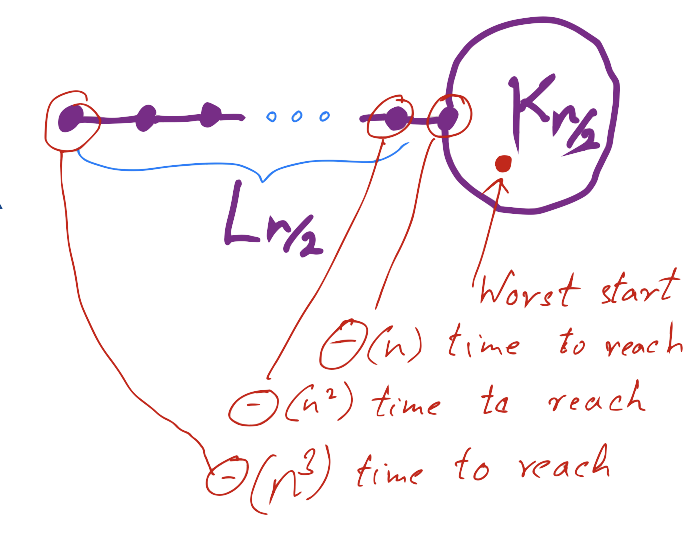
\includegraphics[width=.6\textwidth]{figures/lollipop.png}
    \caption{A lollipop graph $\lollipop_n$ and its cover time.}
    \label{fig:lollipop}
  \end{figure}
\end{itemize}

\begin{theorem} \label{thm:cover}
  Let $G$ be an undirected graph. Then\footnote{When the context is clear, we denote $m = |E|$ in a graph $G = (V, E)$.}
  $$ C(G) \leq O(mn). $$
\end{theorem}

\begin{definition}
  Consider a random walk on a graph $G = (V, E)$. For $x, y \in V$, the \emph{commute time} $C_{x, y} = C_{x, y}(G)$ is defined to be the expected number of steps for the random walk to start at $x$, hit $y$ and return to $x$.
\end{definition}

\begin{proposition}
  For $x, y \in V$,
  $$ C_{x, y} = h_{x, y} + h_{y, x}. $$
\end{proposition}

\begin{proof}
  This is due to linearity of expectation.
\end{proof}

\begin{lemma}
  Consider a random walk on a connected undirected graph $G = (V, E)$. For each $(x, y) \in E$,
  $$ C_{x, y} \leq O(m). $$
\end{lemma}

\begin{proof}
  Construct a graph $G'$ by adding a self-loop at each vertex with probability $1/2$. Let $x, y \in V$. We claim that $C_{x, y}(G') = 2C_{x, y}(G)$. To see this, for each path from $x$ to $y$ in $G'$, removing the self-loops in the path gives a path in $G$, and the expected fraction of self-loops in the path is $1/2$. Then $G'$ is ergodic. This implies that there exists a unique stationary distribution $\pi^*$.

  Consider a walk $u_1, u_2, \ldots$, where $u_i \in V$ and $(u_i, u_{i + 1}) \in E$ for each $i \in \NN$. We look for commutes of the form
  $$ x \to y \to \ldots \to x \to y. $$
  For each $i \in \NN$,
  $$ \PP\left[u_i = x, u_{i + 1} = y\right] = \PP\left[u_i = x\right] \cdot \PP\left[u_{i + 1} = y \;\middle|\; u_i = x\right] = \frac{d(x)}{2m} \cdot \frac{1}{d(x)} = \frac{1}{2m}. $$
  Therefore, the expected fraction of $x \to y$ equals $1/(2m)$. This implies that the expected gap between the $(x \to y)$'s equals $2m$. This proves that $C_{x, y}(G) = O(m)$.
\end{proof}

\begin{proof}[Proof of Theorem \ref{thm:cover}]
  Let $T$ be a spanning tree of $G$. Let $(v_0, v_1, \ldots, v_{2n - 2})$ be a DFS traversal of $T$. For instance, $(1, 2, 3, 2, 4, 2, 1, 5, 1)$ is a DFS traversal of the tree given in Figure \ref{fig:dfs}. Then
  $$ C(G) \leq \sum_{i = 0}^{2n - 3} h_{v_i, v_{i + 1}} = \sum_{(x, y) \in E(T)} C_{x, y} \leq (n - 1) \cdot O(m) = O(mn). $$
  This completes the proof.

  \begin{figure}[h]
    \centering
    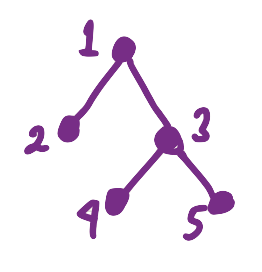
\includegraphics[width=.3\textwidth]{figures/dfs.png}
    \caption{$(1, 2, 3, 2, 4, 2, 1, 5, 1)$ is a DFS traversal of the tree in the figure.}
    \label{fig:dfs}
  \end{figure}
\end{proof}

\section{Unconnected $s$-$t$ Connectivity}

\begin{problem}[undirected $s$-$t$ connectivity, $\ustconn$]
  Given an undirected graph $G = (V, E)$ and $s, t \in V$, output ``yes'' if $s$ and $t$ are in the same connected component of $G$, and ``no'' otherwise.
\end{problem}

\begin{definition}
  Let $\RL$ be the class of problems solvable by randomized log-space computations.
\end{definition}

The computational model that we consider consists of a read-only input tape of $n$ bits and a read-write tape of $O(\log n)$ bits.

\begin{theorem}
  $\ustconn \in \RL$.
\end{theorem}

\begin{proof}
  Let $G = (V, E)$ be an undirected graph. By Theorem \ref{thm:cover}, $C(G) = O(nm) = O(n^3) = cn^3$ for some constant $c$. We give Algorithm \ref{alg:ustconn} for some parameter $k$.

  \begin{algorithm}
    starting at $s$, take a random walk for $k \cdot c n^3$ steps \\
    \If{ever see $t$}{
      \Return{``yes''}
    }
    \Else{
      \Return{``no''}
    }
    \caption{A randomized algorithm for $\ustconn$ on an undirected graph $G = (V, E)$ and vertices $s, t \in V$.}
    \label{alg:ustconn}
  \end{algorithm}

  The running time of Algorithm \ref{alg:ustconn} is $O(n^3)$ times the time to pick a random neighbor (which depends on the specific data structure used). For the space of Algorithm \ref{alg:ustconn}, we need to keep track of the step counter, which uses $O(\log n)$ space, and need to pick a random neighbor, which uses $O(\log n)$. Therefore, Algorithm \ref{alg:ustconn} uses $O(\log n)$ space in total.

  Now we analyze the behavior of Algorithm \ref{alg:ustconn}. If $s$ and $t$ are not connected, then the algorithm never outputs ``yes.'' If $s$ and $t$ are connected, then $h_{s, t} \leq C(G_S) \leq n^3$, where $G_S$ is the connected component of $G$ that contains $s$ and $t$. Therefore,
  \begin{align*}
    \PP[\text{output ``no''}] &\leq \PP[\text{start at $s$, walk at least $k \cdot h_{s, t}$ steps and still don't see $t$}] \\
    &= \PP[\text{start at $s$, walk at least $k \cdot \EE[\text{\# steps to start at $s$ and see $t$}]$ steps, not see $t$}] \\
    &\leq \frac{1}{k}.
  \end{align*}
  Note that the last inequality follows from Markov's inequality. This completes the proof.
\end{proof}

\section{Mixing Time}

We first review some definitions and results from linear algebra.

\begin{definition}
  A vector $v$ is said to be an \emph{eigenvector} of a matrix $A$ with corresponding \emph{eigenvalue} $\lambda$ if $vA = \lambda v$.
\end{definition}

\begin{definition}
  The \emph{$L_2$-norm} of a vector $v = (v_1, \ldots, v_n)$ is defined to be $\sqrt{\sum_{i = 1}^n v_i^2}$.
\end{definition}

\begin{definition}
  A set of vectors $v^{(1)}, \ldots, v^{(m)}$ is said to be \emph{orthonormal} if for all $i, j \in [m]$,
  $$ v^{(i)} \cdot v^{(j)} = \left\{
    \begin{array}{ll}
      1, & \text{if $i = j$}, \\
      0, & \text{if $i \neq j$},
    \end{array}
  \right. $$
  where $v^{(i)} \cdot v^{(j)}$ is the \emph{inner product} of $v^{(i)}$ and $v^{(j)}$, defined to be $\sum_{\ell = 1}^n v_\ell^{(i)} v_\ell^{(j)}$.
\end{definition}

Let $P$ be the transition matrix of the random walk on a $d$-regular undirected graph. Then $P$ is doubly stochastic. Therefore,
\begin{align*}
  \left(\frac{1}{n}, \ldots, \frac{1}{n}\right) \cdot P &= 1 \cdot \left(\frac{1}{n}, \ldots, \frac{1}{n}\right), \\
  \left(\frac{1}{\sqrt{n}}, \ldots, \frac{1}{\sqrt{n}}\right) \cdot P &= 1 \cdot \left(\frac{1}{\sqrt{n}}, \ldots, \frac{1}{\sqrt{n}}\right).
\end{align*}
This shows that $(1/n, \ldots, 1/n)$ and $(1/\sqrt{n}, \ldots, 1/\sqrt{n})$ are eigenvectors of $P$ with eigenvalue $1$. Note that the $L_2$-norm of $(1/\sqrt{n}, \ldots, 1/\sqrt{n})$ equals $1$.

\begin{theorem}
  Let $P$ be an $n \times n$ transition matrix that is real and symmetric. Then there exist eigenvectors $v^{(1)}, \ldots, v^{(n)}$ that form an orthonormal basis with corresponding eigenvalues $\lambda_1, \ldots, \lambda_n$ such that
  $$ 1 = \lambda_1 \geq \left|\lambda_2\right| \geq \ldots \left|\lambda_n\right|, $$
  and that
  $$ v^{(1)} = \frac{1}{\sqrt{n}}(1, \ldots, 1). $$
\end{theorem}

\begin{proposition} \label{prop:eig}
  Let $P$ be a matrix with all positive entries, vectors $v^{(1)}, \ldots, v^{(n)}$, and corresponding eigenvalues $\lambda_1, \ldots, \lambda_n$.
  \begin{enumerate}[itemsep=0pt, label=(\roman*)]
    \item \label{item:scalar} For all $\alpha \in \RR$, $\alpha P$ has eigenvectors $v^{(1)}, \ldots, v^{(n)}$ and corresponding eigenvalues $\alpha \lambda_1, \ldots, \alpha \lambda_n$.
    \item \label{item:id} $P + I$ has eigenvectors $v^{(1)}, \ldots, v^{(n)}$ and corresponding eigenvalues $\lambda_1 + 1, \ldots, \lambda_n + 1$.
    \item For all $k \in \ZZ_+$, $P^k$ has eigenvectors $v^{(1)}, \ldots, v^{(n)}$ and corresponding eigenvalues $\lambda_1^k, \ldots, \lambda_n^k$.
    \item If $P$ is stochastic, then $|\lambda_i| \leq 1$ for all $i \in [n]$.
  \end{enumerate}
\end{proposition}

Note that \ref{item:scalar} and \ref{item:id} in Proposition \ref{prop:eig} imply that $(P + I)/2$ has eigenvectors $v^{(1)}, \ldots, v^{(n)}$ and corresponding eigenvalues $(\lambda_1 + 1)/2, \ldots, (\lambda_n + 1)/2$.

\begin{proof}
  \begin{enumerate}[itemsep=0pt, label=(\roman*)]
    \item Note that $vP = \lambda v$ if and only if $v \cdot \alpha P = \alpha \lambda \cdot v$.
    \item Note that $v(P + I) = vP + vI = \lambda v + v = (\lambda + 1)v$.
    \item Note that $vP^k = (vP)P^{k - 1} = \lambda vP^{k - 1} = \lambda (vP)P^{k - 2} = \lambda^2 vP^{k - 2} = \ldots = \lambda^k v$.
    \item Let $i \in [n]$. Let $I = \{ j \in [n] : v_j^{(i)} > 0 \}$. Then
    \begin{align*}
      \lambda_i \sum_{j \in I} v_j^{(i)} &= \sum_{j \in I} \sum_{k = 1}^n v_k^{(i)} P_{k, j} \\
      &\leq \sum_{j, k \in I} v_k^{(i)} P_{k, j} && (\text{entries of $v$ with coordinates not in $I$ are at most $0$, $P_{k, j} \geq 0$}) \\
      &= \sum_{k \in I} v_k^{(i)} \sum_{j \in I} P_{k, j} \\
      &\leq \sum_{k \in I} v_k^{(i)}. && \left(\text{$\sum_{j \in I} P_{k, j} \leq 1$ since $P$ is stochastic}\right)
    \end{align*}
    Therefore, $\lambda_i \leq 1$.
  \end{enumerate}
\end{proof}

Note that if $v^{(1)}, \ldots, v^{(n)}$ form a basis, then any vector $w$ can be expressed as a linear combination of $v^{(1)}, \ldots, v^{(n)}$, i.e., $w = \sum_{i = 1}^n \alpha_i v^{(i)}$ for some $\alpha_1, \ldots, \alpha_n \in \RR$, and
$$ \| w \|_2 = \sqrt{w \cdot w} = \sqrt{\sum_{i = 1}^n \alpha_i v^{(i)} \sum_{j = 1}^n \alpha_j v^{(j)}} = \sqrt{\sum_{i = 1}^n \sum_{j = 1}^n \alpha_i \alpha_j v^{(i)} v^{(j)}} = \sqrt{\sum_{i = 1}^n \alpha_i^2}. $$
Note that the last equality follows from the orthonormality of $v^{(1)}, \ldots, v^{(n)}$.

Mixing times study the following question: How long does it take to reach the stationary distribution?

\begin{definition}
  For $\varepsilon > 0$, the \emph{mixing time} $T(\varepsilon)$ of a Markov chain $A$ with stationary distribution $\pi$ is the minimum $t \in \ZZ_+$ such that for all initial distribution $\pi^{(0)}$,
  $$ \left\| \pi - \pi^{(0)} A^t \right\|_1 < \varepsilon. $$
\end{definition}

\begin{theorem} \label{thm:mixing}
  Let $P$ be the transition matrix of the random walk on an undirected, $d$-regular and unconnected graph with the greatest common divisor of cycle lengths equal to $1$. Let $\pi_0$ be an initial distribution. Let $\pi$ be the stationary distribution equal to $(1/n, \ldots, 1/n)$ (so $\pi P  = P$). Then
  $$ \left\| \pi_0 P^t - \pi \right\|_2 \leq \left|\lambda_2\right|^2. $$
\end{theorem}

Note that the bound $|\lambda_2|^t$ is good (i.e., exponentially decreasing) if $1 - \lambda_2 = \Theta(1)$.

\end{document}
